\section{Methods}

The institutional review board has approved the study, and all patients have
given written informed consent. The MR examinations were performed between March
2013 and May 2014. The study enrolled 72 consecutive patients with
histologically confirmed PCa who were scheduled for robotic assisted
laparoscopic prostatectomy.

Two of the patients had the Gonadotropin releasing hormone antagonist
(Degarelix, Ferring Pharmaceuticals) started just before the MR examination. The
rest of the patients had no prostate-related hormonal, surgical, or radiotherapy
treatment before or during imaging.

A subset of the data has already been used in previous studies. DWI data sets
(12 b values, 0--2000 s/mm²) of 48 patients were used for evaluating
mathematical models of DWI \citep{Toivonen2015, Jambor2015Relaxation,
Jambor2015Evaluation}, while T₂ of 37 patients were used in feasibility
evaluation of relaxation along fictitious field and continuous wave T₁ᵨ imaging
of PCa \citep{Jambor2015Relaxation, Jambor2015Rotating}.

The data sets, post-processing program code as well as all MR sequences are
freely available upon request following acceptance of the manuscript.


\subsection{MRI examination}

The MR examinations, as previously described \citep{Jambor2015Evaluation,
Toivonen2015, Jambor2015Relaxation}, were performed using a 3T MR scanner
(Ingenuity PET/MR, Philips, Cleveland, USA), a two channel volume whole body RF
coil for excitation, and a 32 channel manufacture's cardiac coils for measuring
the signal.

Transversal single shot turbo spin echo (TSE) T₂-weighted images (T₂w) were
acquired with repetition time/echo time (TR/TE) 4668/130 ms, field of view (FOV)
250×250 mm², matrix size 250×320, slice thickness 2.5 mm, no intersection gap,
and SENSE \citep{Pruessmann1999} factor~2. The acquisition time was 1~min 10~s.

For acquiring the DWI data sets, a single shot spin-echo based sequence was used
with monopolar diffusion gradient scheme and echo-planar read out. Other
parameters were TR/TE 3141/51 ms, FOV 250×250 mm², acquisition matrix 100×99,
reconstruction matrix 224×224, slice thickness 5.0 mm, number of slices 20,
intersection gap 0.5 mm, diffusion gradients applied in three directions,
diffusion gradient timing ($\Delta$) 24.5 ms, diffusion gradient duration
($\delta$) 12.6 ms, diffusion time ($\Delta-\delta/3$) 20.3 ms, SENSE
\citep{Pruessmann1999} factor~2, partial-Fourier acquisition 0.69, SPAIR fat
suppression, and b~values (number of signal averages) 0 (2), 100 (2), 300 (2),
500 (2), 700 (2), 900 (2), 1100 (2), 1300 (2), 1500 (2), 1700 (3), 1900 (4),
2000 (4) s/mm². The acquisition time was 8~min 48~s.

T₂ relaxation values (T₂ mapping) were obtained using a gradient and spin echo
(GraSE) sequence with TR/TEs of 686/20, 40, 60, 80, 100 ms, FOV 230×183 mm²,
acquisition matrix 256×163, reconstruction matrix 512×400, slice thickness 5.0
mm, and no intersection gap. The acquisition time was 1~min 35~s.


\subsection{Histopathological analysis and cancer delineation on MRI}

The whole mount prostatectomy sections were processed as previously described
\citep{Jambor2015Evaluation, Jambor2015Rotating}. The hematoxylin-eosin stained
histological slides were first reviewed by one staff board certified pathologist
and later re-reviewed by one experienced genitourinary pathologist (PT). In the
cases there were differences between the two reviews, the opinion of the third
genitourinary pathologist was searched and consensus was reached between the
involved genitourinary pathologists.

The histology slice thickness of whole mount prostatectomy sections was
approximately 4 mm (range 4--6 mm). Gleason scores were assigned to tumors as
combinations of primary, secondary, and tertiary Gleason grade, as defined by
the 2005 International Society of Urological Pathology Modified Gleason Grading
System \citep{Epstein2005}. If a Gleason grade pattern higher than the primary
and secondary grade was present and visually accounted for less than 5\% of the
tumor volume, it was assigned as tertiary Gleason grade \citep{Epstein2010}.

Prostate cancer extent on each MRI acquisition (T₂w, DWI, T₂) was manually
delineated by one research fellow (IJ) working in consensus with the
genitourinary pathologist (PT), using whole mount prostatectomy sections as
``ground truth.'' Anatomical landmarks were used to align each MRI acquisition
(T₂w, DWI, T₂) with mount prostatectomy sections.


\subsection{Final data set}

Ten of the patients were excluded from further analysis due to presence of
motion (n=2), severe susceptibility artifacts (n=5), or incomplete data (n=3).
The characteristics of the remaining 62 patients are shown in Supporting
Material (Table S1). Their median age was 65 years (range 45--73 years), while
the median serum PSA value was 9.3 ng/ml (range 1.3--30.0 ng/ml). The number of
patients having one, two, and three lesions was 29, 28, and 5, respectively.

The final data set was composed of 100 PCa lesions derived from the MRI data
sets of these 62 patients. In total, 67 and 33 lesions were located in
peripheral zone (PZ) and central gland (CG), respectively. For the purpose of
classifier performance evaluation, the Gleason scores of prostate cancer lesions
were divided into two groups of low (3+3) and high (>3+3), containing 20 and 80
lesions, respectively.


\subsection{MRI data post-processing}

The post-processing pipeline is outlined in Fig~\ref{fig:pipeline}. An
example case with resulting standardized image and fitted parametric maps is
shown in Fig~\ref{fig:pmap}. The in-house software used in fitting was
quality controlled for correctness with cross-comparison to independent
implementation and with visual inspections of parametric maps and distributions.

\begin{figure}[!ht]
    \centering
    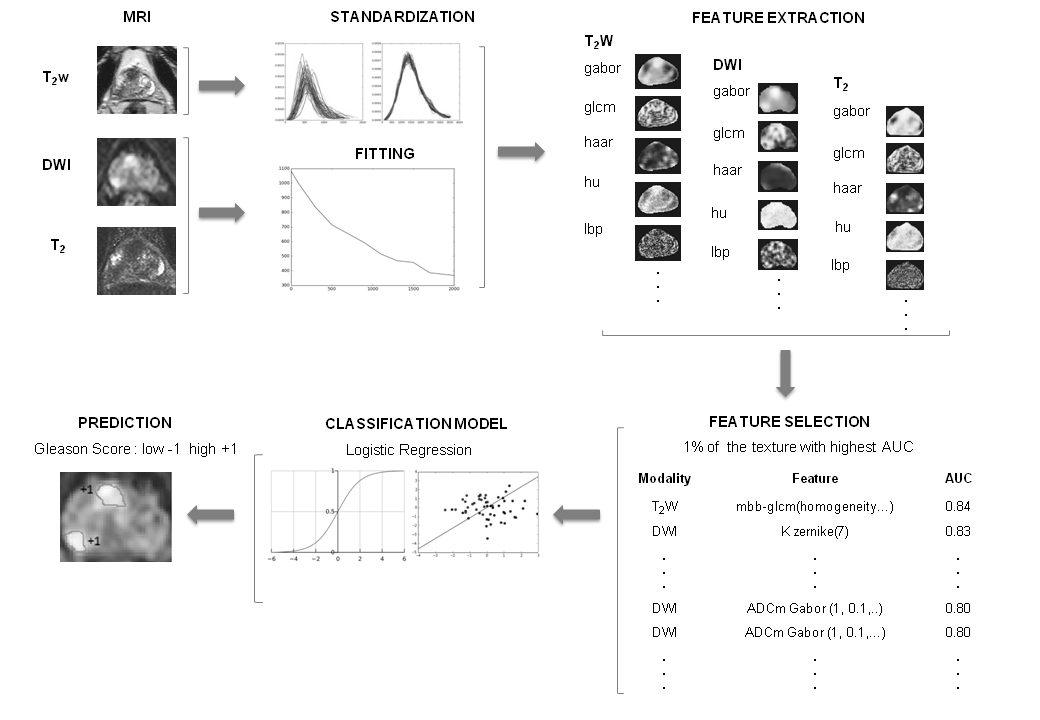
\includegraphics[width=1.0\textwidth]{figures/fig1}
    \caption{{\bf The post-processing pipeline.}
    The T₂-weighted imaging (T₂w) data set is standardized, while the
    monoexponential and kurtosis models are applied to diffusion weighted
    imaging (DWI) data set. The T₂ relaxation values are obtained using a two
    parameter monoexponential function. Subsequently, the features are
    calculated using T₂w and parametric maps. The feature selection is performed
    by choosing 1\% of the features with highest AUC\@. Then with the selected
    features a logistic regression model is fitted and used to predict the
    lesion's Gleason score group.}%
    \label{fig:pipeline}
\end{figure}

\begin{figure}[!ht]
    \centering
    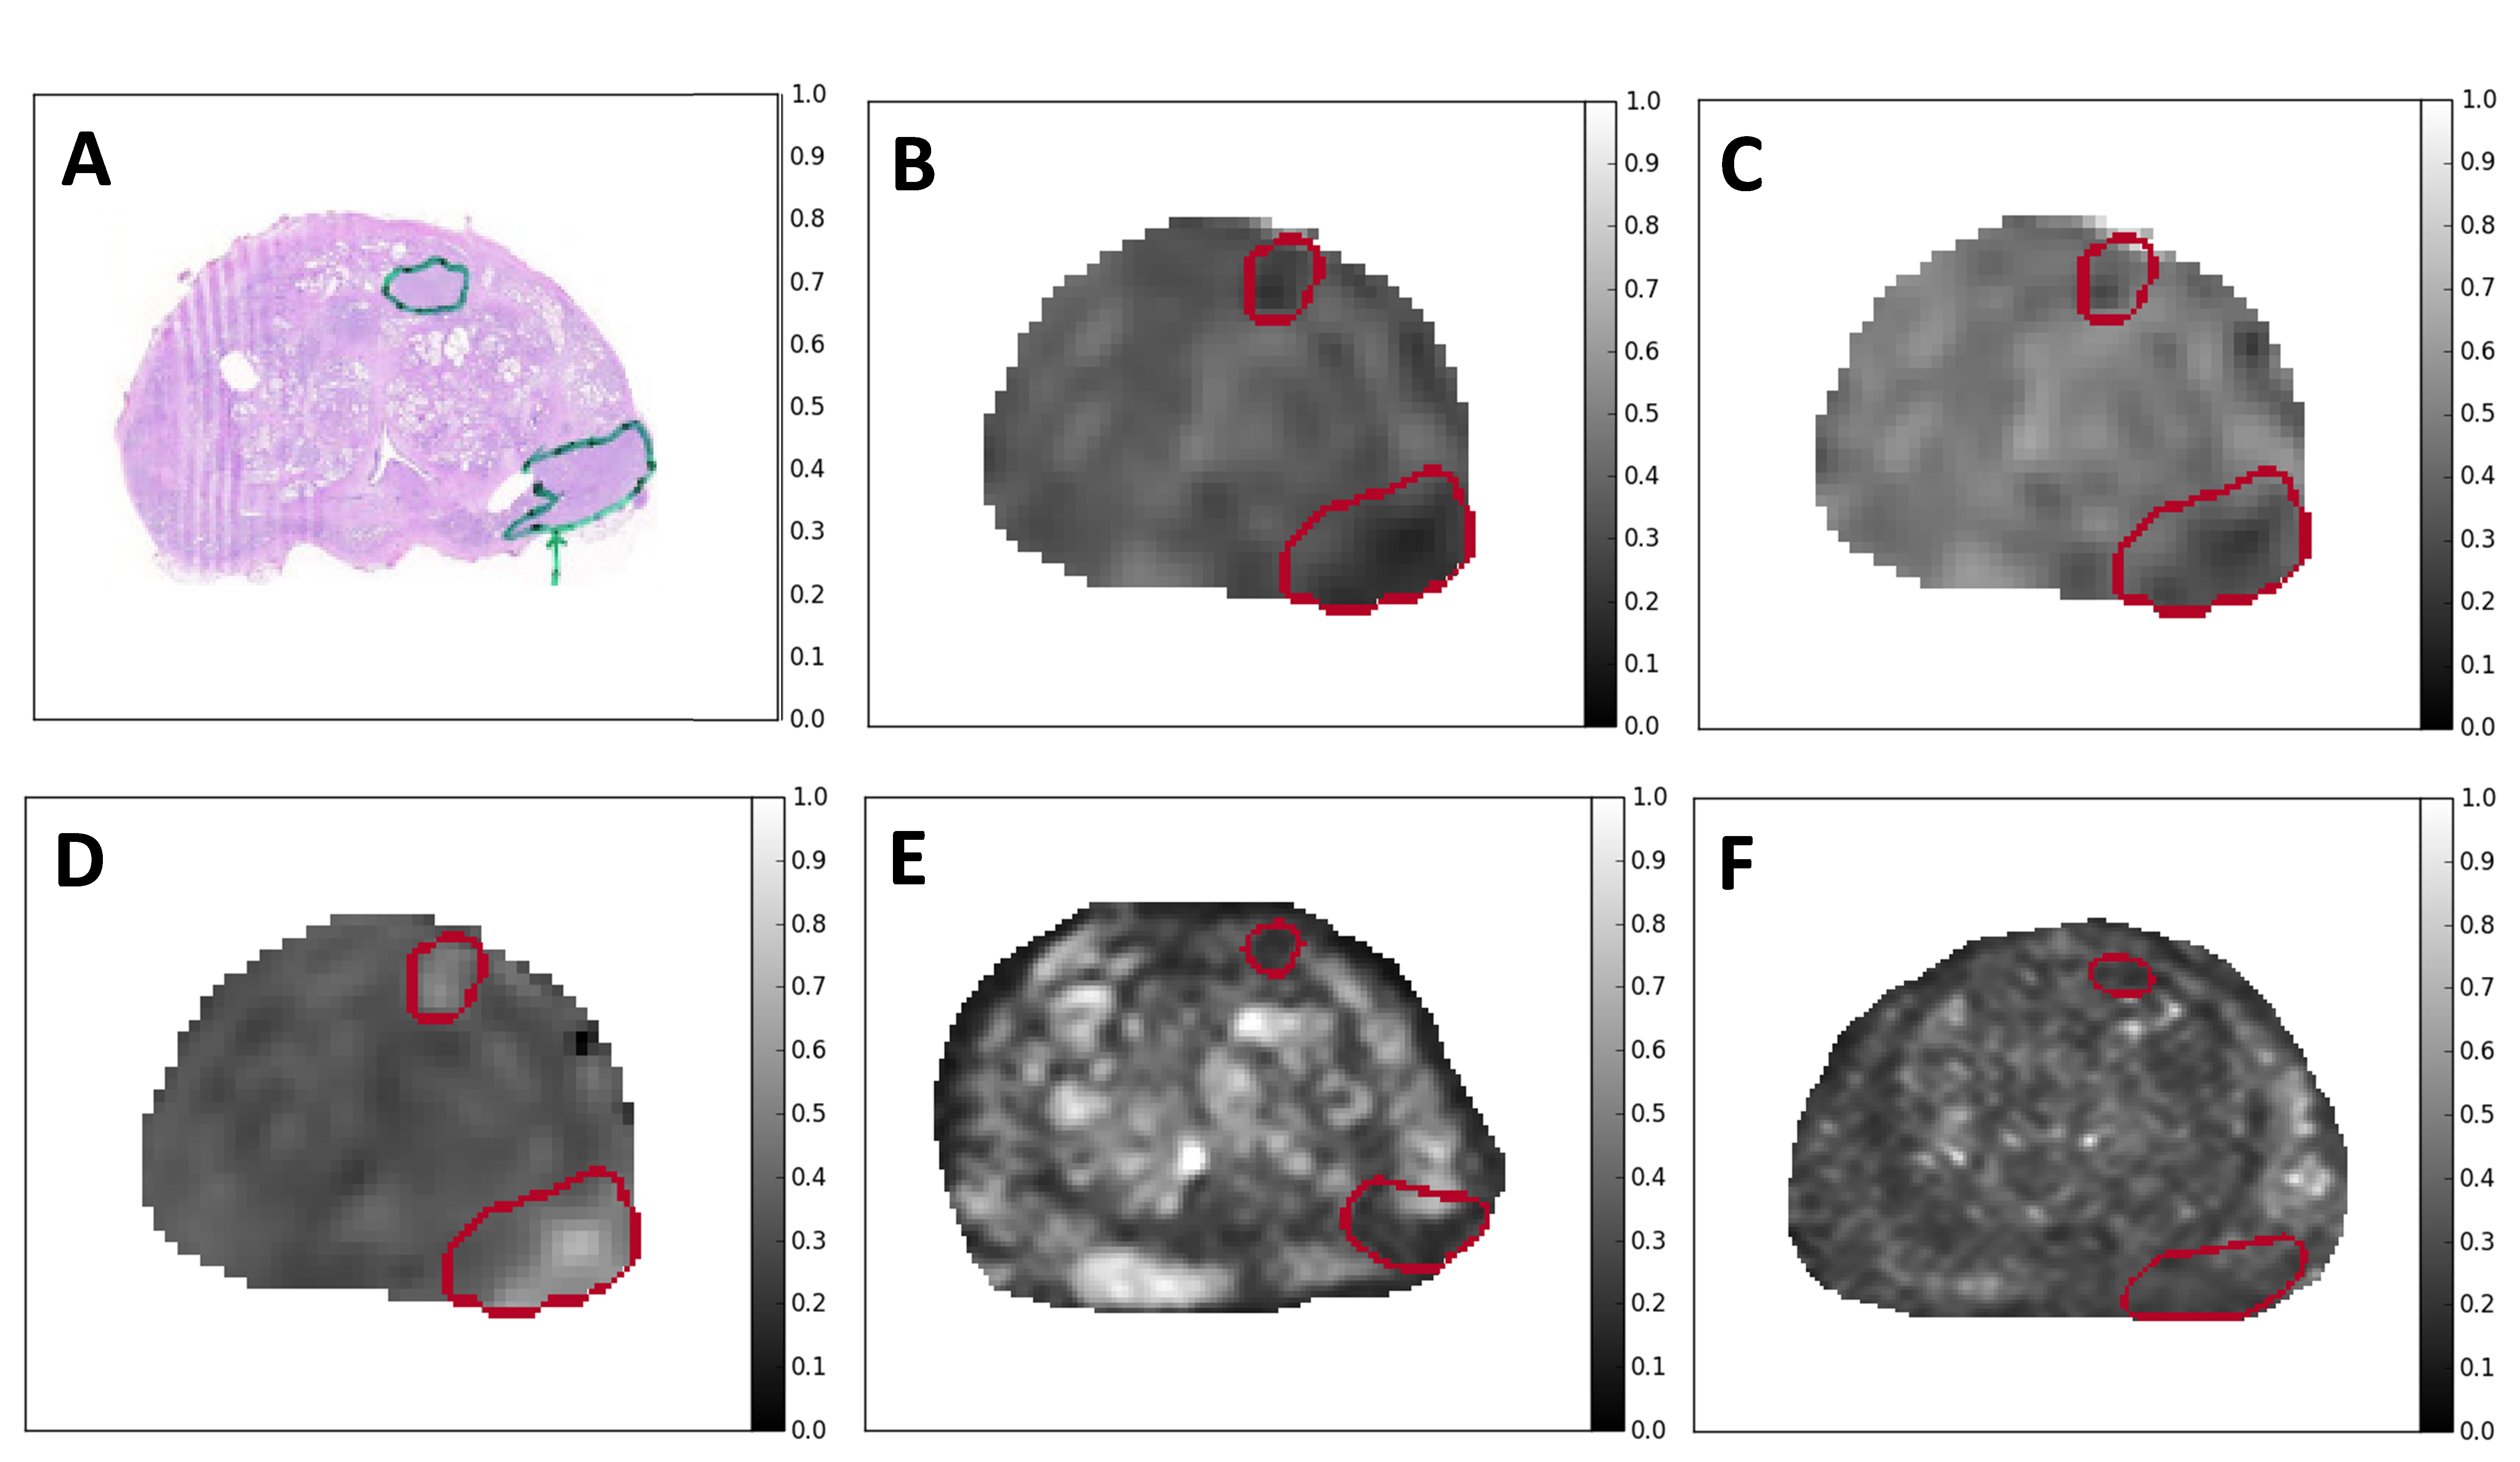
\includegraphics[width=1.0\textwidth]{figures/fig2}
    \caption{{\bf An example case with parametric maps.}
    A:~Whole mount prostate histological section.
    B:~ADCₘ. C:~ADCₖ. D:~K. E:~T₂w. F:~T₂.
    This is from patient \#43 in Table~S1. The two lesions are outlined; their
    Gleason scores are 4+3 (lower, posterolateral region) and 3+4 (upper,
    anterior region).}%
    \label{fig:pmap}
\end{figure}

\subsubsection{T₂w standardization}

The signal intensity of a T₂w image is not a specific tissue property and
this non-standardness of T₂w images (``intensity drift'') requires
standardization to a common scale. To correct this bias, a histogram alignment
method was used, as described by Nyúl et al.\ \cite{Nyul1999, Nyul2000}. This
simple method transforms the images to make their histograms match at certain
landmark locations, and interpolates the values between.

In this study, the deciles (i.e.\ every tenth percentile) were used as
landmarks, as suggested by Nyúl et al.\ \cite{Nyul1999}. Only delineated
prostate volume was considered for histogram averages, as other parts of the
image might distort the learning. The result was validated by visual inspection.

\subsubsection{DWI fitting}

Diffusion weighted imaging data sets were fitted on voxel level using the
monoexponential model:

\begin{equation}
  S(b) = S_0 \exp(-b \text{ADCₘ})
\end{equation}

and the kurtosis model \citep{Jensen2005}:

\begin{equation}
  S(b) = S_0 \exp\left(
    -b \text{ADCₖ} + \frac{1}{6} b^2 \text{ADCₖ}^2 \text{K}
  \right)
\end{equation}

where $S(b)$ is the signal intensity as a function of $b$ value, $S_0$ is the
signal intensity at $b=0$~s/mm², ADCₘ is the apparent diffusion coefficient
of the monoexponential model, ADCₖ is the apparent diffusion coefficient of
the kurtosis model, and K is the kurtosis.

The fitting procedure was performed using the Broyden-Fletcher-Goldfarb-Shanno
(BFGS) algorithm \citep{Shanno1985} implemented by the dlib \citep{King2009}
library. In order to find a reliable fit and prevent local minima, the algorithm
was executed with multiple evenly spaced initialization values. Their intervals
(step sizes) were for ADCₘ 0.1--3.0~µm²/ms (0.01~µm²/ms), for ADCₖ
0.01--3.0~µm²/ms (0.1~µm²/ms), and for K 0.0001--4.0 (0.2).

\subsubsection{T₂ fitting}

T₂ relaxation values were calculated on a single voxel level using a two
parameter monoexponential function:

\begin{equation}
  S(\TE) = S_0 \exp(-\TE / \text{T₂})
\end{equation}

where $S(\TE)$ is the signal intensity at given time $\TE$, $S_0$ is the signal
intensity at $\TE=0$~ms, and T₂ is the spin-spin relaxation time.

The Levenberg-Marquardt algorithm was used for fitting, as implemented by the
SciPy library, with the multiple initialization values of 0.0~ms to 300~ms with
step size of 50~ms. T₂ relaxation values were constrained to 1--300~ms interval.


\subsection{Feature extraction}

Texture extraction methods can be roughly categorized into four main groups
\citep{Castellano2004}, although this taxonomy is somewhat ambiguous. The
statistical approach is based on local spatial distributions and relationships
of intensity occurrences in the image. The structural methods use well-defined
geometrical primitives to measure texture. The model-based methods attempt to
represent the image properties as parameters of various mathematical models. The
transform methods use signal processing transformations such as Fourier and
wavelets to analyze the image in a different space.

In this study, the gray-level co-occurrence matrix, the local binary patterns,
and the histogram of oriented gradients can be assigned into the statistical
category, and the Sobel operator into the structural one. The Hu and Zernike
moments belong to the model-based group, while the Gabor filter and the Haar
wavelet are transform methods.

The selection of texture extraction methods used in this study was based mainly
on prior experiences in existing MRI literature \citep{Castellano2004,
Lemaitre2015} and the availability of applicable open-source software
components. All of these texture descriptor methods, except the Hu and Zernike
moments, have been previously used for CAD of PCa. However, detailed information
on their implementation and parameter selection are usually very scarce. This
issue was addressed in this study by providing complete information on the
parameters, and by using a wide array of them.

Three-dimensional texture extraction of MRI has been utilized in various
studies, including some of PCa diagnosis \citep{Depeursinge2014}. In this study,
however, texture analysis was performed only in 2D and per-slice, due to voxel
anisotropy.

\subsubsection{General implementation details}

Several texture descriptor methods with various parameter combinations were used
for extracting 2D texture features from the manually delineated PCa lesions.
Most of the methods in this study inherently incorporate the so-called ``sliding
window'' algorithm. This means that the local voxel neighborhood for
calculations is represented as a fixed-shape subwindow centered at each voxel in
turn. The output image, a texture feature map, consists of the feature values
positioned on corresponding neighborhood center locations. A more detailed
explanation is provided by Clausi et al.\ \cite{Clausi2002Rapid}, for example.

Seven window configurations were used for DWI and nine for T₂w and T₂
data. These square-shaped windows had evenly spaced voxel side lengths of 3, 5,
…, 15 for DWI and 3, 7, …, 35 for the higher-resolution T₂w and T₂. These
lengths correspond to 3.3--17 mm for DWI and 1.4--16 mm for T₂w and T₂,
maintaining similar physical cover over different resolutions.

For each lesion, the window was placed on all possible locations along the
transverse planes so that it still stayed completely within the lesion area. In
cases of the window not fitting completely inside lesion area, the window
locations with maximum lesion area were used. Extracted texture feature maps
were then averaged over all slices to be used as lesion-wise median features.
The use of different window sizes and parameter combinations resulted in 1281
features per DWI image type (ADCₘ, ADCₖ, K) and 1631 features per other image
type (T₂w, T₂), totaling 7105 features all five image types combined. The free
software libraries Scikit-image \citep{VanderWalt2014} and Mahotas
\citep{Coelho2013} were utilized in the implementation of the process.

\subsubsection{Method-specific implementation details}

The gray-level co-occurrence matrix (GLCM) \citep{Haralick1973} is a very
popular method of texture characterization. It observes all the pixel gray level
pairings that occur in the image at a certain distance and direction. In this
study, the GLCM was calculated for each window using four different voxel
distances of 1 to 4 (unless prevented by window dimensions). Because the 22
GLCM-derived features introduced by Haralick et al.\ \cite{Haralick1973} have
correlation \citep{Albregtsen2008}, using only three to five features have been
recommended \citep{Clausi2002Analysis, Albregtsen2008, Gebejes2013a} in order to
minimize redundancy and dimensionality.

In this study, the six GLCM features implemented by the Scikit-image software
library \citep{VanderWalt2014} were extracted. These features, namely contrast,
dissimilarity, homogeneity, energy, correlation, and angular second moment
(i.e.\ uniformity), are among the ones most commonly used in previous studies
\citep{Clausi2002Rapid}. They are generally considered effective texture
discriminators, and maintain invariance regarding scale and shift
\citep{Clausi2002Analysis}. In order to gain orientation invariance, the results
were averaged over four bidirectional axes, and mean range over the orientations
was added \citep{Haralick1973}.

Since GLCM requires a discrete source image, the images needed prior
normalization depending on source type. All images were quantized by uniform
scaling to 32 gray levels, based on previous studies \citep{Clausi2002Analysis,
Clausi2002Rapid, Albregtsen2008}. The image type specific source intensity
ranges for scaling were manually defined by observing prostate volume
histograms. In total 324--420 GLCM related features with sliding window approach
were extracted per image type (T₂w, ADCₘ, ADCₖ, K, T₂).

In addition to the sliding window approach, the same GLCM-based features were
also extracted using the minimum bounding box (MBB) around the whole lesion
area of each image slice as the window, while ignoring any non-lesion voxels.
This procedure is similar to the method used in a study by Vignati et
al.\ \cite{Vignati2015}. The MBB-GLCM features were averaged over slices, and
48 features in total were extracted per image type.

Local binary patterns (LBP) \citep{Ojala1996} is a method that compares every
voxel intensity value to a certain number of neighboring values on a circle
around it. Each comparison result is stored as a single bit that tells whether
the neighbor is larger or smaller than the center. The bit patterns are
collected from the neighborhood and encoded as numbers, and the resulting
histogram can then be used as a feature vector invariant to gray scale. In this
study, the LBP were calculated within each window, observing eight interpolated
neighboring points at the maximum radius allowed by window size. The different
orientations of the uniform patterns were combined into rotation-invariant
groups, and all non-uniform patterns were treated as a single pattern. Pattern
frequency histograms were then used as features resulting in 70--90 different
features per image type.

The Gabor function \citep{Gabor1946} is a Gaussian modulated by a sinusoidal
wave. Gabor filter banks can be used for texture characterization, as each
filter, shaped by its parameters, responds to specific local spatial frequency
properties of the image \citep{Turner1986}. Gabor filters are sensitive to edges
in the image, so given that different lesions contain different regions, the
detected edges between the regions could yield different responses. In this
study, the texture extraction scheme described by Tüceryan et
al.\ \cite{Tuceryan1998} was applied, which uses the sliding window on the
Gabor-filtered complex images.

Based on experimentation and data visualization, the filter bank included the
combinations of five different frequencies for the sinusoidal
($f=0.1,0.2,…,0.5$ per voxel), three sizes for a circular Gaussian
envelope ($\sigma=1,2,3$), and four bidirectional orientations. A number of
derived features have been suggested \citep{Clausi2000, Hammouda2000,
Grigorescu2002}. Here, the extracted features included mean of the real part,
variance of the real part, mean of the absolute of the real part, and mean of
the magnitude. Various ways to achieve orientation invariance have been proposed
\citep{Arivazhagan2006, Han2007, Chu2009, Rahman2011}, although not all are
equally suitable for texture classification. In this study, the simple method of
summing filtered images over orientations was used \citep{Han2007}, yielding
420--540 features per image type.

The Haar transform is a simple wavelet decomposition of the image. Providing
local spatial frequency information, it is useful as a tool of texture analysis
\citep{Lonnestad1992}. In this study, a four-level Haar transform was first done
for each image slice, and the three higher frequency coefficient planes were
used, upscaled to the original size. For each sliding window, the mean absolute
value and the standard deviation were then extracted as features
\citep{Lonnestad1992}, resulting in 168--216 features per image type.

Image moments are weighted averages that describe the distribution of intensity
within image. A few variations are widely used as object shape descriptors, but
they have also been applied to texture analysis \citep{Tuceryan1994}. In this
study, logarithms of the absolute values of the seven Hu moments \citep{Hu1962},
and the magnitude values of the complex Zernike moments \citep{Teague1980} up to
the 8th degree were calculated for each window. The Hu moments are invariant
regarding translation, scaling, rotation, and reflection
\citep{Theodoridis2003}. The Zernike moment magnitudes are rotation invariant,
robust to noise, and, due to their orthogonality, have minimal redundancy
\citep{Tahmasbi2011, Amayeh2005}. In total, 49--63 Hu moments and 175--225
Zernike moments were extracted from each image type.

The histogram of oriented gradients \citep{Dalal2005} is an algorithm developed
primarily for object recognition. It describes an object as a set of local
gradient direction distributions. In this study, it was applied for texture
analysis, using a single cell with eight directions for each window. The average
over windows was then used as a feature, resulting in one feature per window
size and 7--9 features in total per image type.

The Sobel operator \citep{Sobel1990} is a simple convolution filter that
emphasizes edges in image. The shape of the kernel window is 3×3 by definition,
so no other window sizes were used. Instead, the median of the whole lesion-wide
texture map was used, both with the lesion edge voxels included and excluded,
resulting in 2 features.

In addition, first-order statistical features were calculated over the whole
lesion. First-order statistics observe only the probabilistic distribution of
intensity values, ignoring their spatial relations. Existing literature
typically utilizes averages and some of the percentiles \citep{Shaish2016}.
Here, 18 features were included, namely mean, standard deviation, range,
minimum, maximum, quartiles, deciles, kurtosis, and skewness.


\subsection{Classification}

For image types ADCₘ, ADCₖ, and K, a corresponding data set of 100 data points and
1281 features were used to build models for predicting prostate lesion
aggressiveness based on Gleason score, while for T₂w and T₂ the number of
features was 1631. The features were normalized to zero mean and unit variance.
The data points were divided into two groups by Gleason score, low and high
(3+3 and >3+3, respectively).

Logistic regression with either L1 or L2 regularization \citep{Friedman2010}
implemented by Python Scikit-learn library \citep{Pedregosa2011} were used to
train the low vs high Gleason score classifiers. Both regularization mechanisms
compensate the high dimensionality of the data by penalizing large coefficient
values of the inferred linear models, which in turn makes them less likely to
overfit to the training data and more able to generalize to data unseen in the
training phase.

L1 regularization has the additional property of shrinking the coefficients of
the least useful features down to zero, and hence it also performs feature
selection \citep{Park2007}. The number of coefficients ending down to zero
depends on the amount of regularization. However, regularizing too strongly
might lose valuable features and lead to underfitting. Therefore, it was also
tested whether the simultaneous use of the classical filtering based feature
selection approach would improve the prediction performance.

The predictive performance of the models built by the regularized logistic
regression algorithms was estimated by a nested cross validation strategy
\citep{Varma2006}, which consisted of an outer leave-pair-out cross-validation
(LPOCV) \citep{Airola2011} and an inner 10-fold cross validation (10FCV) for
hyperparameter selection. In LPOCV every possible pair of data points were held
out at a time as test set, while the remaining data formed the training set used
to build the model for predicting on the held out pair. Both the filter based
feature selection and the hyperparameter selection were performed for each
round on LPOCV using the training set.

For selecting the best features, their performance was estimated using the
receiver operating characteristic (ROC) curve, summarized as the area under the
ROC curve (AUC). Ranked by AUC, the highest-performing 1\% of the features were
used to train the classifier.

After selecting the features the training set was transformed accordingly and
the optimum regularization hyperparameter value was selected from $\omega =
\{0.001, 0.01, 0.1, 1, 10\}$, as measured by the AUC in stratified 10FCV\@. A
classifier was then trained with the selected features and the regularization
hyperparameter, and used for performing predictions on the two data points held
out during the LPOCV round.

Afterwards, each data point was assigned an LPOCV score according to the
ordering-by-the-number-of-wins method, in which the score of a data point is the
number of times it obtains a larger predicted value than the other point during
the LPOCV rounds when it is one of the two held out points. These LPOCV scores
were then used to perform the ROC curve analysis, whose validity was previously
demonstrated by Balcan et al.\ \cite{Balcan2008}. More precisely, using the
LPOCV scores of the data points and their corresponding true label, the AUC and
95\% confidence interval (CI) were calculated using the R package by LeDell et
al.\ \cite{LeDell2015}.

The feature selection and hyperparameter selection process as part of the LPOCV
is illustrated in Pseudo code~\ref{alg:pseudocode}. The algorithm starts with a
loop referred as LPOCV\@. During this loop the indices associated with the test
pair in turn, $(i,j)$ with $i \neq j$, are not included in the index set $C$ of
training data. Every feature AUC is calculated using data from matrix $\vec{X}$
and label vector $\vec{y}$. The notation $\vec{X}[C,k]$ refers to the submatrix
of $\vec{X}$ containing the rows indexed by $C$ and the columns by $k$, that is,
the vector with the values for $k$th feature in the training data. The top 1\%
independent features are indexed by $\indx$. The optimum regularization
hyperparameter value $\alpha \in \omega$ is calculated using 10FCV on data
$(\vec{y}[C], \vec{X}[C,\indx])$, which is then used to train a model $f$ to
make predictions on the test pair $(\vec{X}[i,\indx], \vec{X}[j,\indx])$. The
last line of the pseudo code describes the calculation of LPOCV score using
ordering-by-the-number-of-wins method.

\begin{algorithm}[!h]
  \caption{{\bf LPOCV with inner feature selection by AUC filtering and
  hyperparameter selection.}}%
  \label{alg:pseudocode}

  \begin{algorithmic}
    \REQUIRE{$\vec{X}$, matrix of $n$ lesions × $F$ features}
    \REQUIRE{$\vec{y}$, vector of labels (1 high, -1 low)}
    \REQUIRE{$\omega = \{0.001, 0.01, 0.1, 1, 10\}$, set of hyperparameters}
    \ENSURE{LPOCV scores}
    \FOR[All possible lesion pairs]{$i, j \in \{1,2,\dotsc,n\}$}
      \STATE{$C \gets \{1,2,\dotsc,n\} \setminus \{i,j\}$}
          \COMMENT{All lesions except $i,j$}
      \STATE{$\vec{auc} \gets$ vector of length $F$}
      \FOR{$k \in \{1,2,\dotsc,F\}$}
        \STATE{$\vec{auc}[k] \gets \mathrm{AUC}(\vec{X}[C,k], \vec{y}[C])$}
            \COMMENT{Calculate AUC for each feature}
        \STATE{$\vec{auc}[k] \gets \max(\vec{auc}[k], 1-\vec{auc}[k])$}
            \COMMENT{Handle inverse correlation}
      \ENDFOR{}
    \STATE{$\indx \gets \arg\mathrm{sort}(\vec{auc})[1 \dotso (0.01 \times F)]$}
        \COMMENT{Get indices of the best features}
    \STATE{$\alpha \gets \mathrm{gridSearch}(\vec{y}[C], \vec{X}[C,\indx], \omega)$}
        \COMMENT{Grid search with 10FCV, returns the best hyperparameter}
    \STATE{$f \gets A(\vec{y}[C], \vec{X}[C,\indx], \alpha)$}
        \COMMENT{Train model f with algorithm A and hyperparameter $\alpha$}
    \STATE{$\vec{W}_{ij} \gets H(f(\vec{X}[i,\indx]) - f(\vec{X}[j,\indx]))$}
        \COMMENT{Matrix W stores results from Heaviside function (H) of i and j
        prediction difference}
    \ENDFOR{}
    \STATE{$\tilde{\vec{y}} \gets \vec{W} \textbf{1}$}
        \COMMENT{Score of each element obtained by summing along axis j}
    \RETURN{$\tilde{\vec{y}}$}
        \COMMENT{Returns LPOCV scores}
  \end{algorithmic}
\end{algorithm}


\subsection{Addressing bias and imbalance}

It is important to note that the nested cross-validation scheme allows feature
selection and hyperparameter tuning while avoiding bias in the performance
estimate \citep{Varma2006}. In each round of LPOCV, the pair of data points left
for testing does not affect the feature selection nor the hyperparameter tuning
of the predictive model in turn.

The ratio between low and high Gleason score is 1:4 in the data set, so there is
some degree of imbalance between classes. However, the model performance was
estimated using LPOCV together with AUC, and that degree of imbalance in the
classes has low effect on these methods \citep{Airola2011, Smith2014}. LPOCV is
an unbiased estimate of the prediction performance of a model
\citep{Airola2011}, and the ROC AUC is not affected by imbalance as it measures
how accurately a model ranks a random positive unit from a negative one
\citep{Fawcett2006}.
